\documentclass{article}
\usepackage[a4paper,top=0.75in, bottom=0.75in, left=1in, right=1in,footskip=0.2in]{geometry}
%\usepackage{fullpage}
%-----------------Hyperlink Packages--------------------
\usepackage{hyperref}
\hypersetup{
	 colorlinks   = true,
     citecolor    = black,
     linkcolor    = black,
     urlcolor     = black
}
%-----------------Figure Packages--------------------
\usepackage{graphicx}                       % For figures
%\usepackage{epsfig} % for postscript graphics files
%------------------Math Packages------------------------
\usepackage{amssymb,amsmath}
\usepackage{textcomp}
\usepackage{mdwmath}
\usepackage{mdwtab}
\usepackage{eqparbox}
%------------------Table Packages-----------------------
\usepackage{rotating}                     % Used to rotate tables
\usepackage{array}                        % Fixed column widths for tables
%-----------------Algorithm Packages--------------------
\usepackage{listings}                     % Source code
\usepackage{algorithm}                    % Pseudo Code
\usepackage{algpseudocode}
%---------------------------------------------------------

%opening

\begin{document}

\title{
Artificial Intelligence Project 2 \\
Decision Tree
}
\author{Class 1, Team 6}
\date{\today}
\maketitle

\section{Team Members}

\begin{table}[H]
\centering
\begin{tabular}{l l l}
Name & Student ID  & Job\\
\hline
Fan Ziyao & 12330081 & Team leader, implementation\\
Chen Yingcong & 12330049 & Implementation \\
Chen Xiongtao & 12330040 & Modeling, implementation \\
Huang Long & 12330132 & Implementation \\
Zhang Qiuyi & 12330402 & Implementation, documentation

\end{tabular}
\end{table}

\section{Problem Description}

The dataset contains the records of the United States congressional votes in 1984. There are 435 records, each containing the party (goal attribute) of the congressman/congresswoman and his/her votes on 16 bills. There are only two types of values for the goal attribute: `democrat' and `republican', and three types for other attributes: `n' (can be considered as nay), `y' (can be considered as yea), and `?' (can be considered as missing).

Given this dataset, the goal is to build a decision tree to classify a record (that is, to find out the party of this congressman/congresswoman) according to its known attributes (that is, his/her votes on these 16 bills). Both the training set and the testing set will be sampled from this dataset.

\section{Algorithm and Implementation}

For this project we implemented the C4.5 algorithm to build the decision tree. Since the dataset only have two effective values (`y' and `n') for all attributes, there is no need to use the information gain ratio as the measure of attributes. The information gain alone is more suitable for this dataset.

To handle the missing data, when building the tree, we only consider the records with defined value for the attribute being measured. When classifying the record, we use the probability of each possible value to weigh the calculation of each branch.

The data set is split by sampling the training set with a given probability $p$. The rest of the data will be put in to the testing set.

\subsection{Decision tree building}

The algorithm for building the decision tree is described in Algorithm~\ref{alg:build}.

Since the decision tree built with this data set won't be very deep (after all, there are only 16 attributes, and the data set is fairly skewed), a recursive implementation is sufficient. Records with missing values of the chosen attribute will be ignored when calculating the information gain.

\begin{algorithm}[H]
\centering
\caption{Decision tree bulding}
\label{alg:build}
  \begin{algorithmic}[1]
    \Function{Build}{$data$, $attributes$}
        \If{$data$ is empty}
        	\State \Return an empty node
        \EndIf
        \State $gain_{best}$ = 0.0, $attr_{best}$ = None
        \State $value_{best}$ = None, $sets_{best}$ = None
	    \For{each attribute $a$ in $attributes$}
    		\State Divide $data$ based on values of $a$ into $set1$, $set2$
    		\State Calculate the information gain of spliting $data$ into $set1$ and $set2$, ignoring missing values
    		\If{The new information gain $> gain_{best}$}
    			\State Update $gain_{best}$, $attr_{best}$, $sets_{best}$, $value_{best}$
    		\EndIf
	    \EndFor
	    \If{$attributes$ is not empty and $gain_{best} \neq 0.0$}
	    	\State remove $attr_{best}$ from $attributes$
	    	\State $left\_branch =$ \Call{Build}{$set1$ in$ sets_{best}$, $attributes$}
	    	\State $right\_branch =$ \Call{Build}{$set2$ in$ sets_{best}$, $attributes$}
	    	\State Create a node $node$
	    	\State $node.attr = attr_{best}$, $node.value = value_{best}$
	    	\State $node.left = left\_branch$, $node.right = right\_branch$, $node.count$ = size of $data$
	    	\State \Return $node$
      	\Else
      		\State Create a node $node$
      		\State $node.leaves = $ count of each parties in $data$
      		\State $node.count = $ size of $data$
      		\State \Return $node$
      	\EndIf
    \EndFunction
  \end{algorithmic}
\end{algorithm}

\begin{description}
\item Remark 1. \hfill \\
The \textit{entropy} of a attribute $V$ in the data set $D$ is defined as:

$$
H(V, D) = -\sum_k P(v_k) \log_2\frac{1}{P(v_k)}
$$

where $v_k$ are values of $V$ in $D$, $P(v_k)$ is the probability of $v_k$ in $D$.

\item Remark 2.\hfill \\
When a data set $D$ with goal attribute $V$ is split into subsets $D_k$ using attribute $A$, each with $n_k$ records, the \textit{information gain} is defined as:

$$
Gain(A) = H(V, D) - Remainder(A)
$$

where

$$
Remainder(A) = \sum_k P(n_k) H(V, D_k)
$$

$P(n_k)$ is the proportion of $E_k$ in $D$.
\end{description}

\subsection{Decision tree pruning}

The algorithm for pruning the decision tree is described in Algorithm~\ref{alg:prune}. For the same reason as the tree building, a recursive implementation is enough. Nonetheless, since the data set is quite skewed, there is seldom a need for pruning the tree.

\begin{algorithm}[H]
\centering
\caption{Decision tree pruning}
\label{alg:prune}
  \begin{algorithmic}[1]
    \Function{Prune}{$tree$, $min\_gain$}
    	\If{$tree.left$ is not a leave}
    		\State\Call{Prune}{$tree.left$, $min\_gain$}
    	\EndIf
    	\If{$tree.right$ is not a leave}
    		\State\Call{Prune}{$tree.right$, $min\_gain$}
    	\EndIf
    	\If{Both $tree.left$ and $tree.right$ are leaves}
    		\State Temprorily combine $tree.left$ and $tree.right$ into $new\_node$
    		\State $delta = \Call{Entropy}{new\_node}-  (\Call{Entropy}{tree.left} + \Call{Entropy}{tree.right}) / 2$
    		\If{$delta < min\_gain$}
    			\State Replace $tree$ with $new\_node$
    		\EndIf
    	\EndIf
    \EndFunction
  \end{algorithmic}
\end{algorithm}

\subsection{Classification}

The algorithm for classifying an observation is described in Algorithm~\ref{alg:cla}. It follows all branches at any node for which a value is missing and multiply the weights along each path.

\begin{algorithm}[H]
\centering
\caption{Classification}
\label{alg:cla}
  \begin{algorithmic}[1]
    \Function{Classify}{$tree$, $observation$}
    	\If{$tree$ is a leave}
    		\State\Return $tree.leaves$
    	\EndIf
    	\State $value$ = $observation[tree.attr]$
    	\If{$value$ is missing}
    		\State $result\_left =  \Call{Classify}{tree.left, observation}$
    		\State $result\_right =  \Call{Classify}{tree.right, observation}$
    		\State $weight\_left = tree.left.count/tree.count$
    		\State $weight\_right = tree.left.count/tree.count$
    		\For{each pair of $goal, count$ in $result\_left$}
    			\State$result[goal] += count * weight\_left$
    		\EndFor
    		\For{each pair of $goal, count$ in $result\_right$}
    			\State$result[goal] += count * weight\_right$
    		\EndFor
    		\State \Return $result$
    	\Else
    		\If{$value = tree.left.value$}
    			\State \Return \Call{Classify}{$tree.left$, $observation$}
    		\Else
    			\State \Return \Call{Classify}{$tree.right$, $observation$}
    		\EndIf
    	\EndIf
    \EndFunction
  \end{algorithmic}
\end{algorithm}

\section{Experiment Result}

To evaluate the implementation, we sample the data with probability $p$ and use the sample as training set. The rest of the data set will be the testing set. One of the decision tree built with $p = 0.2$ is visualized in Figure~\ref{fig:tree}. In addition, we take training sets sampled with various $p$ to generate the learning curve for evaluation, as shown in Figure~\ref{fig:curve}. With training sets of different sizes, the precisions of cross validation fluctuate between $0.9$ and $1.0$, with mean $\mu = 0.9462$ and standard variation $\sigma = 0.0175$.

\begin{figure}[H]
\centering
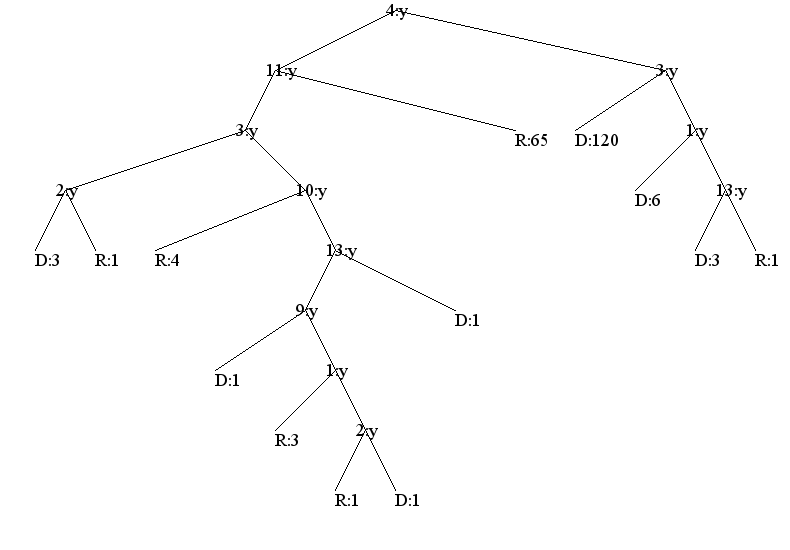
\includegraphics[width=400pt]{../asset/tree.png}
\caption{One of the decision trees built with training set sampled with $p = 0.5$}
\label{fig:tree}
\end{figure}

\begin{figure}[H]
\centering
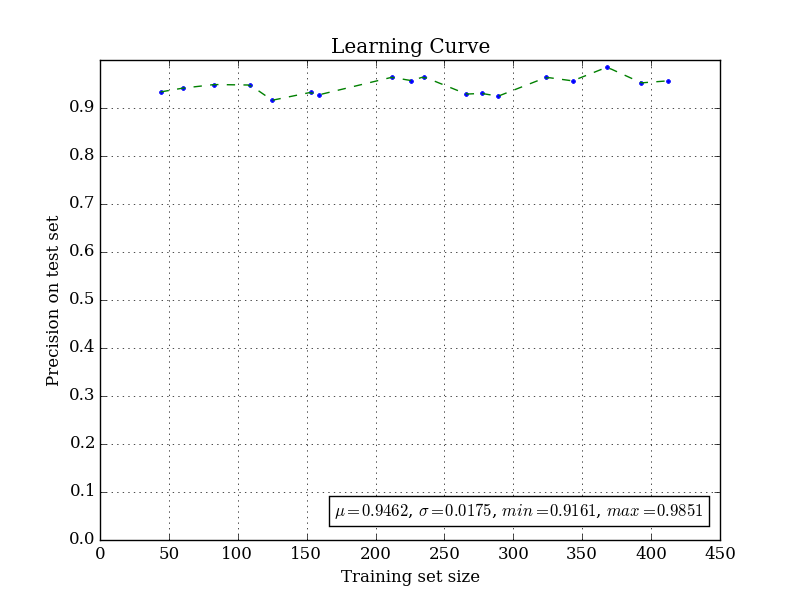
\includegraphics[width=400pt]{../asset/learning-curve.png}
\caption{Learning Curve}
\label{fig:curve}
\end{figure}

\end{document}
